\documentclass[12pt]{article}

\usepackage{sbc-template}
\usepackage{graphicx,url}
\graphicspath{{figuras/}}
\usepackage[utf8]{inputenc}
\usepackage[T1]{fontenc}
\usepackage[brazil]{babel}
\usepackage{booktabs}
\usepackage{amsmath}

\sloppy

\title{Avaliação de Predição de Desvios no HeapSort em {RISC-V} com o Simulador gem5}

\author{Matheus H. R. da Costa\inst{1}, Lucas S. Schuch\inst{1}, Kassiara R. Bosing\inst{1},\\
  Jean C. C. Gondorek\inst{1}, Jonathan G. Correa\inst{1}}

\address{Universidade Federal da Fronteira Sul (UFFS)\\
  Chapecó -- SC -- Brasil
  \email{\{matheus.dacosta, lucas.schuch, kassiara.bosing\}@estudante.uffs.edu.br}
  \email{\{jean.gondorek, jonathan.correa\}@estudante.uffs.edu.br}
}

\begin{document}

\maketitle

\begin{abstract}
  This work evaluates branch prediction techniques on a HeapSort algorithm implemented in RISC-V assembly and simulated with gem5. As required by the assigned topic, two predictors --- LocalBP (local, simple) and BiModeBP (global bi-mode) --- are compared on an \emph{in-order} (TIMING) pipeline, measuring the total number of evaluated branches and misprediction counts extracted from \texttt{stats.json}. With an identical set of evaluated branches, BiModeBP reduces mispredictions by about 38\% (and 45\% on the data-dependent \texttt{DirectCond} branches of \texttt{heapify}), improving prediction accuracy where purely local predictors struggle.
\end{abstract}

\begin{resumo}
  Este trabalho avalia t{\'e}cnicas de predi{\c{c}}{\~a}o de desvios no HeapSort implementado em assembly RISC-V e simulado no gem5. Conforme o t{\'o}pico escolhido, dois preditores --- LocalBP (local simples) e BiModeBP (bi-mode global) --- s{\~a}o comparados em pipeline \emph{em-ordem} (TIMING), medindo o total de desvios avaliados e a quantidade de predi{\c{c}}{\~o}es incorretas extra{\'i}das de \texttt{stats.json}. Com o mesmo conjunto de desvios avaliados, o BiModeBP reduz as predi{\c{c}}{\~o}es erradas em cerca de 38\% (e 45\% nos desvios condicionais diretos \texttt{DirectCond} da rotina \texttt{heapify}), melhorando a precis{\~a}o onde preditores puramente locais t{\^e}m dificuldade.
\end{resumo}

\section{Introdução}

No Trabalho 1 da disciplina de Organização de Computadores, validou-se a corretude funcional de um HeapSort em RISC-V utilizando simuladores instrucionais (Venus). Neste trabalho, o mesmo algoritmo é analisado sob a ótica de microarquitetura com o simulador de ciclo de clock gem5 \cite{binkert2011gem5}, conforme especificação da atividade \cite{uffs2026org}.

O tópico escolhido é \textbf{Predição de Desvios} (tópico 2): comparar \texttt{LocalBP} com \texttt{BiModeBP} \cite{lee1997bi}, ambos no modelo \emph{em-ordem} (\texttt{TIMING}), conforme exigido pelo enunciado, medindo o total de desvios avaliados e a quantidade de erros de predição. O HeapSort apresenta laços regulares e desvios dependentes de dados em \texttt{heapify}, sendo um caso de estudo adequado.

\section{Fundamentação Teórica}

\subsection{Predição de desvios}

Em pipelines com múltiplos estágios, instruções de desvio condicional exigem que o processador preveja o próximo endereço de execução antes que a condição seja resolvida \cite{hennessy2017computer}. Predições incorretas geram \emph{bubbles}: ciclos perdidos enquanto o pipeline é refeito a partir do endereço correto. O \textbf{LocalBP} mantém um histórico de desvios por endereço de instrução (PC); é eficiente quando o mesmo PC tem comportamento estável, mas sofre com \emph{aliasing} entre PCs distintos. O \textbf{BiModeBP} combina um preditor local com escolha por PC e um preditor global, separando padrões predominantemente taken e not-taken, o que reduz o aliasing em código com mistura de laços e comparações.

\subsection{Desvios no HeapSort}

O HeapSort implementado utiliza \emph{min-heap} e produz ordenação decrescente \emph{in-place}. Os pontos críticos de desvio são:

\begin{itemize}
  \item \textbf{Laços regulares}: \texttt{build\_loop} e
        \texttt{extract\_loop} executam comparações de contador
        (\texttt{blt}/\texttt{ble}) com padrão previsível.
  \item \textbf{Comparações em \texttt{heapify}}: instruções
        \texttt{blt} comparam valores do vetor; o resultado depende dos
        \textbf{dados}, dificultando preditores puramente locais.
  \item \textbf{Chamadas recursivas}: \texttt{jal}/\texttt{ret} geram
        desvios de chamada/retorno, geralmente bem previstos pela Return
        Address Stack (RAS).
\end{itemize}

\section{Metodologia}

\subsection{Ambiente e compilação}

O código assembly \texttt{heapSort\_original.s} foi adaptado do Trabalho~1 para a sintaxe GCC, com ponto de entrada \texttt{main}, uso de \texttt{printf} e alocação via \texttt{malloc}. A compilação gera binário estático exigido pelo gem5:

\begin{verbatim}
riscv64-linux-gnu-gcc -static heapSort_original.s \
  -o heapSort_original.riscv
\end{verbatim}

As simulações foram executadas em ambiente Docker com gem5 (\texttt{gem5.opt}) e o script \texttt{inorder.py}. Todos os cenários usam a CPU \texttt{CPUTypes.TIMING} (pipeline em-ordem) com cache L1 de 32\,kB, L2 de 256\,kB, memória DDR3 de 1\,GB e clock de 3\,GHz; a comparação entre preditores de desvio (\texttt{LocalBP} vs.\ \texttt{BiModeBP}) mantém os demais parâmetros de hardware idênticos entre os dois cenários.

\subsection{Geração assistida das simulações}

Pedimos a um modelo de LLM que reescrevesse \texttt{inorder.py} aceitando, via \texttt{argparse}, CPU, preditor de desvio, clock, caches L1/L2, hierarquia, núcleos e memória, parametrização usada para fixar os valores padrão (CPU \texttt{TIMING}, 3\,GHz, L1 32\,kB, L2 256\,kB, DDR3 1\,GB) na comparação dos preditores. Executamos a comparação com o vetor padrão ($n=6$) e, para validar o comportamento em escala maior, também com $n=100.000$ elementos, gerado pela IA em assembly puro a partir de \texttt{heapSort\_gem5.s}; ambas as execuções usam os mesmos valores padrão do \texttt{inorder.py}.

\subsection{Cenários experimentais}

Dois cenários foram comparados mantendo-se idênticos os demais parâmetros de hardware:

\begin{itemize}
  \item \textbf{Cenário A}: \texttt{LocalBP} --- preditor local simples.
  \item \textbf{Cenário B}: \texttt{BiModeBP} --- preditor bi-mode global.
\end{itemize}

O vetor de entrada padrão contém $n = 6$ elementos (\texttt{\{12, 11, 13, 5, 6, 7\}}). Complementarmente, executou-se a mesma comparação com $n = 100\,000$ elementos, também na CPU \texttt{TIMING} a 3\,GHz, para validar o comportamento em escala maior.

\subsection{Métricas coletadas}

As estatísticas foram extraídas do arquivo \texttt{m5out/stats.json} gerado após cada simulação, com foco nas métricas exigidas pelo enunciado:

\begin{itemize}
  \item \texttt{branchPred.BTBLookups} --- total de desvios condicionais avaliados;
  \item \texttt{branchPred.condIncorrect} --- predições incorretas;
  \item \texttt{simTicks} --- tempo total de simulação;
  \item IPC, calculado como \texttt{simInsts / core\_numCycles}.
\end{itemize}

A taxa de erro global foi calculada como $\text{taxa} = \texttt{condIncorrect} / \texttt{lookups}$, ou seja, predições incorretas sobre o total de desvios avaliados. Todas as métricas de \texttt{branchPred} (Figuras~\ref{fig:inorder} e~\ref{fig:escala}) e a Tabela~\ref{tab:baseline} usam a CPU em-ordem (\texttt{TIMING}), conforme o tópico 2 do enunciado.

\section{Resultados}

\subsection{Cenário baseline (3\,GHz, pipeline em-ordem)}

A entrega parcial confirmou a execução correta do binário no gem5. A Tabela~\ref{tab:baseline} resume as métricas do cenário baseline com CPU em-ordem a 3\,GHz.

\begin{table}[ht]
\centering
\caption{Métricas do cenário baseline (CPU em-ordem, 3\,GHz, $n=6$)}
\label{tab:baseline}
\begin{tabular}{lc}
\toprule
\textbf{Métrica} & \textbf{Valor} \\
\midrule
\texttt{simTicks} & 106.596.297 \\
IPC & 0,395 \\
Instruções simuladas (\texttt{simInsts}) & 126.371 \\
Misses L1D & 548 (taxa 1,95\%) \\
\bottomrule
\end{tabular}
\end{table}

\subsection{Comparação LocalBP vs. BiModeBP (pipeline em-ordem)}

A Figura~\ref{fig:inorder} apresenta a comparação direta entre os dois preditores na CPU \texttt{TIMING}, com $n=6$. Como o pipeline em-ordem efetiva os mesmos desvios independentemente do preditor, o total de desvios avaliados (\texttt{lookups}) é idêntico nos dois cenários (30.992); o que muda é a quantidade de erros.

\begin{figure}[ht]
\centering
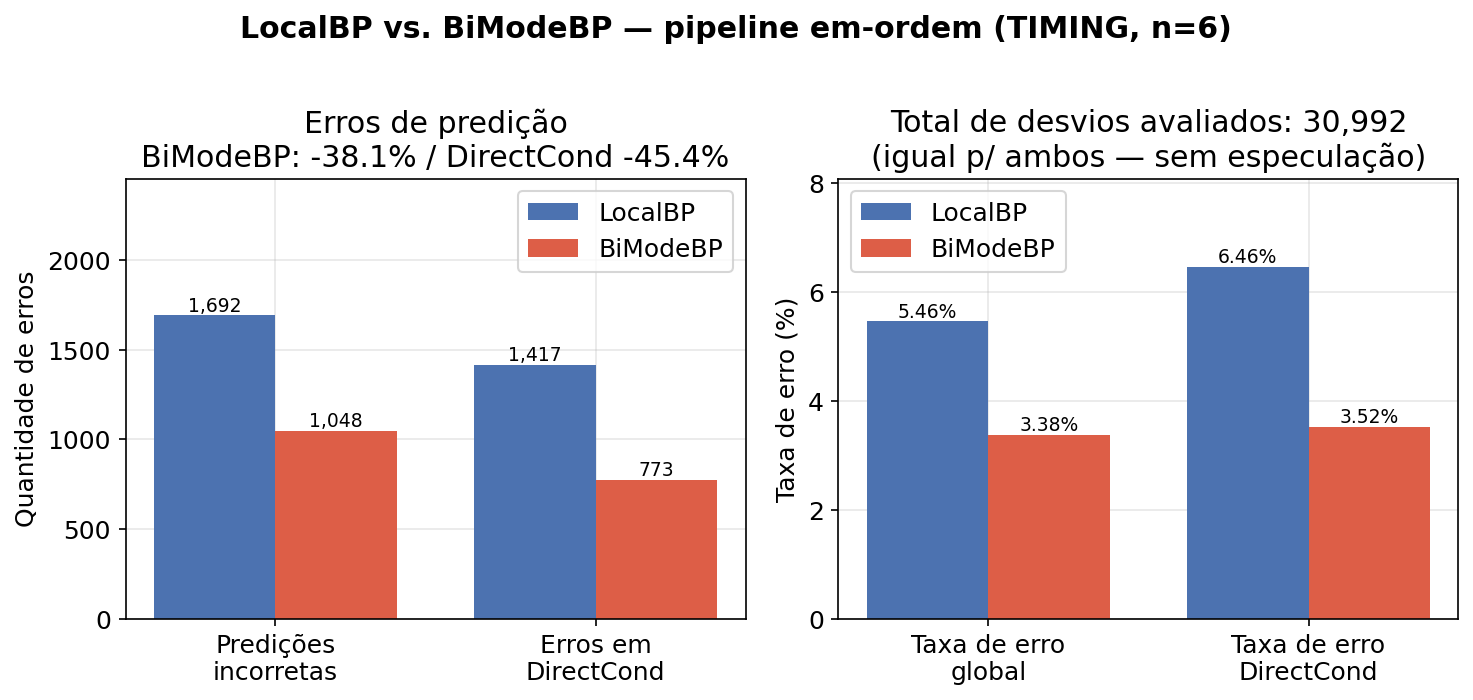
\includegraphics[width=0.95\textwidth]{comparacao_inorder.png}
\caption{Comparação dos preditores em pipeline em-ordem (\texttt{TIMING}, $n=6$): quantidade de erros (esq.) e taxas de erro (dir.).}
\label{fig:inorder}
\end{figure}

O BiModeBP reduziu substancialmente as predições incorretas (\textbf{38,1\%} a menos que o LocalBP), especialmente nos desvios condicionais diretos (\texttt{beq}/\texttt{blt}, \textbf{45,4\%} a menos), que correspondem às comparações em \texttt{heapify} e aos laços de construção e extração do \emph{heap}.

Apesar da redução expressiva nas predições incorretas, o \texttt{simTicks} é \emph{idêntico} entre os dois preditores ($\approx$106,6 milhões): o modelo em-ordem do gem5 mede corretamente quantos erros ocorrem, mas não aplica penalidade de ciclos por \emph{misprediction} no tempo simulado.

\subsection{Efeito de escala (n=100.000)}

Para checar se o padrão observado em $n=6$ se mantém em escala maior, repetimos a comparação com $n=100.000$ na mesma CPU \texttt{TIMING}. A Figura~\ref{fig:escala} mostra a taxa de erro global nas duas escalas: o BiModeBP reduz a taxa de erro em ambas (\textbf{38,1\%} em $n=6$ e \textbf{24,9\%} em $n=100.000$), e o \texttt{simTicks} permanece idêntico entre preditores também em $n=100.000$, confirmando que o efeito é específico do modelo em-ordem, não do tamanho da entrada.

\begin{figure}[ht]
\centering
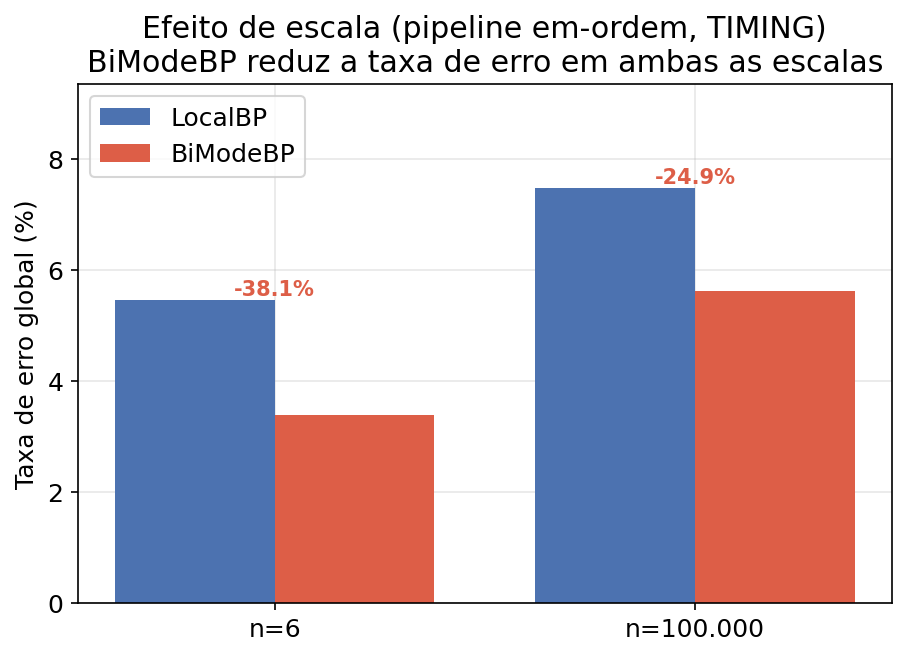
\includegraphics[width=0.80\textwidth]{efeito_escala.png}
\caption{Taxa de erro global (\texttt{condIncorrect}/\texttt{lookups}) em pipeline em-ordem, $n=6$ vs. $n=100.000$.}
\label{fig:escala}
\end{figure}

\section{Discuss{\~a}o}

Os la{\c{c}}os \texttt{build\_loop} e \texttt{extract\_loop} possuem comportamento de desvio estável, sendo bem servidos por ambos os preditores. Já em \texttt{heapify}, cada nó executa até duas comparações \texttt{blt} cujo resultado depende dos valores no vetor; o mesmo endereço de instrução é reexecutado com resultados distintos a cada chamada recursiva, o que eleva \texttt{condIncorrect} no LocalBP. O BiModeBP mitiga esse efeito ao separar históricos taken/not-taken e empregar informação global, reduzindo a taxa de erro em \texttt{DirectCond} de 6,46\% para 3,52\%.

A medição em-ordem responde diretamente ao tópico (quantos desvios e quantos erros), mas não captura o custo desses erros em tempo: o pipeline \texttt{TIMING} do gem5 não modela a penalidade de \emph{misprediction}, por isso o \texttt{simTicks} é idêntico entre os preditores tanto em $n=6$ quanto em $n=100.000$. Conclui-se que, neste modelo, a vantagem do BiModeBP se manifesta em \emph{precisão} (menos erros), não em tempo de execução simulado.

\section{Conclusão}

Para o HeapSort em RISC-V simulado no gem5 em pipeline em-ordem, o preditor \textbf{BiModeBP} adapta-se melhor que o \textbf{LocalBP}. A redução de 38,1\% nas predições incorretas (45,4\% nos desvios condicionais diretos) decorre da maior precisão nos desvios de \texttt{heapify}, onde comparações dependentes de dados desafiam preditores puramente locais. Esse ganho de precisão se mantém em $n=100.000$ (redução de 24,9\%), mas não se traduz em tempo de simulação no modelo \texttt{TIMING}, que não penaliza \emph{mispredictions} em ciclos. Recomenda-se o BiModeBP para cargas com padrão misto de laços regulares e comparações data-dependent; como trabalho futuro, sugere-se repetir a comparação em pipeline fora de ordem para observar o efeito da predição sobre o tempo de execução.

\section*{Declaração de uso de IA}

Ferramentas de inteligência artificial foram utilizadas na reescrita de \texttt{inorder.py} e do HeapSort em escala (\texttt{heapSort\_100k.s}) e na revisão textual deste relatório, conforme descrito na Seção~3.2. A interpretação dos resultados, a execução dos experimentos e a análise microarquitetural são de responsabilidade dos autores.

\bibliographystyle{sbc}
\bibliography{referencias}

\appendix
\section{Comandos de compilação e simulação}
\label{ap:comandos}

\begin{verbatim}
# Compilar o binario estatico RISC-V
riscv64-linux-gnu-gcc -static heapSort_original.s \
  -o heapSort_original.riscv

# Simular no gem5 (CPU em-ordem, baseline)
./gem5/build/RISCV/gem5.opt src/models/inorder.py \
  --binary src/heapSort_original.riscv

# Extrair metricas relevantes
grep -E "simTicks|ipc|branchPred" m5out/stats.json
\end{verbatim}

\section{Trecho de assembly com desvios críticos}
\label{ap:assembly}

\begin{verbatim}
check_left:
    ...
    blt t4, t6, set_left_min    # comparar filho esquerdo
    j check_right
check_swap:
    beq s3, a2, done_heapify    # precisa trocar?
    ...
    jal ra, heapify             # recursao
build_loop:
    blt s3, zero, build_done    # laco de construcao
extract_loop:
    ble s4, zero, extract_done  # laco de extracao
\end{verbatim}

\end{document}
